\documentclass[11pt]{article}
\usepackage[UTF8]{ctex}
\usepackage[a4paper]{geometry}
\geometry{left=2.0cm,right=2.0cm,top=2.5cm,bottom=2.5cm}

\usepackage{caption}
\usepackage{paralist}
\usepackage{enumitem}
\setenumerate[1]{itemsep=0pt,partopsep=0pt,parsep=0pt,topsep=0pt}
\setitemize[1]{itemsep=2pt,partopsep=0pt,parsep=\parskip,topsep=2pt}
\usepackage{comment}
\usepackage{booktabs}
\usepackage{graphicx}
\usepackage{float}
\usepackage{diagbox}
\usepackage{amsmath,amsfonts,graphicx,amssymb,bm,amsthm}
%\usepackage{algorithm,algorithmicx}
\usepackage[ruled, linesnumbered]{algorithm2e}
% \usepackage[linesnumbered]{algorithm2e}
\usepackage[noend]{algpseudocode}
\usepackage{fancyhdr}
\usepackage{tikz}
\usepackage{graphicx}
\usetikzlibrary{arrows,automata, positioning}
\usepackage{hyperref}
\usepackage{extarrows}
% 这是一些字体选项
\usepackage{helvet}
% \usepackage{mathpazo}
\usepackage{fontspec}
% \setmainfont{Times New Roman}
% \setmainfont{Comic Sans MS} % 比较fancy的字体
% \setmainfont{Avenir}
% \setmainfont{Palatino}

% set for automata
\tikzset{
        ->,  % makes the edges directed
        >=stealth, % makes the arrow heads bold
        node distance=2cm, % specifies the minimum distance between two nodes. Change if n
        every state/.style={thick, fill=gray!10}, % sets the properties for each ’state’ n
        initial text=$start$, % sets the text that appears on the start arrow
        }

\setlength{\headheight}{14pt}
\setlength{\parindent}{0 in}
\setlength{\parskip}{0.5 em}


\newtheorem{theorem}{Theorem}
\newtheorem{lemma}[theorem]{Lemma}
\newtheorem{proposition}[theorem]{Proposition}
\newtheorem{claim}[theorem]{Claim}
\newtheorem{corollary}[theorem]{Corollary}
\newtheorem{definition}[theorem]{Definition}
\newtheorem*{definition*}{Definition}

\newenvironment{problem}[2][Problem]{\begin{trivlist}
\item[\hskip \labelsep{\bfseries#1}\hskip\labelsep{\bfseries#2.}]}{\hfill$\blacktriangleleft$\end{trivlist}}
\newenvironment{answer}[1][Answer]{\begin{trivlist}
\item[\hskip \labelsep{\bfseries\itshape#1.}\hskip \labelsep]}{\hfill$\lhd$\end{trivlist}}

\newcommand\E{\mathbb{E}}
\newcommand\per{\mathrm{per}}
% chktex-file 44
% \renewcommand{\familydefault}{\sfdefault}

\title{Homework \#1}
\usetikzlibrary{positioning}

\begin{document}
\captionsetup[figure]{labelfont={bf},name={Fig.},labelsep=period}
\kaishu

\pagestyle{fancy}
\lhead{\CJKfamily{zhkai} Peking University}
\chead{}
\rhead{\CJKfamily{zhkai} Introduction to Theory of Computation, 2024 Spring}

\begin{center}
    {\LARGE \bf Homework 1}\\
    {Name: 方嘉聪\ \  ID: 2200017849}            % Write down your name and ID here.
\end{center}

\begin{problem}{1.(10 points)}
    $~$
\begin{enumerate}[label = (\alph*)]
    \item (5 points) Give a DFA recognizing the following language. The alphabet is $\{0, 1\}$.
    \begin{align*}
        \{w \mid w \mbox{ contains exactly two }0\mbox{s and at least one }1\}
    \end{align*}
    \item (5 points) Give an NFA recognizing the language $0^*1^*0^+$ with four states (including a reject state). The alphabet is $\{0, 1\}$.
\end{enumerate}
\end{problem}
\begin{answer}
    \begin{enumerate}
        \item The DFA shows below:
        \begin{figure}[h]
        \centering
        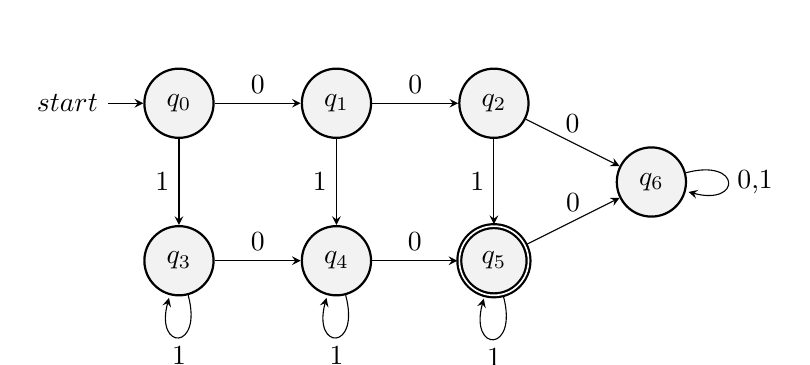
\begin{tikzpicture}
            \node[initial, state] (q0) {$q_0$};
            \node[state, right of=q0] (q1) {$q_1$};
            \node[state, right of=q1] (q2) {$q_2$};
            \node[state, below of=q0] (q3) {$q_3$};
            \node[state, right of=q3] (q4) {$q_4$};
            \node[state, accepting, right of=q4] (q5) {$q_5$};
            \node[state, right of=q2, yshift = -1cm] (q6) {$q_6$};
            \draw (q0) edge[above] node{0} (q1)
                  (q0) edge[left] node{1} (q3)
                  (q1) edge[above] node{0} (q2)
                  (q1) edge[left] node{1} (q4)
                  (q2) edge[left] node{1} (q5)
                  (q2) edge[above] node{0} (q6)
                  (q6) edge[loop right] node{0,1} (q6)
                  (q3) edge[loop below] node{1} (q3)
                  (q3) edge[above] node{0} (q4)
                  (q4) edge[above] node{0} (q5)
                  (q5) edge[above] node{0} (q6)
                  (q5) edge[loop below] node{1} (q5)
                  (q4) edge[loop below] node{1} (q4);
        \end{tikzpicture}
        \end{figure}
        \item The NFA shows below ($q_r$ is the rejecting state, $q_a$ is the accepting state):
        \begin{figure}[h]
        \centering
        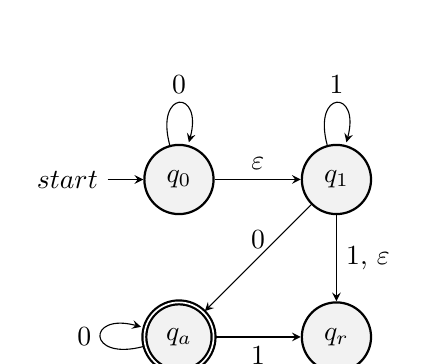
\begin{tikzpicture}
            \node[initial, state] (q0) {$q_0$};
            \node[state, right of=q0] (q1) {$q_1$};
            \node[state, accepting, below of=q0] (a) {$q_a$};
            \node[state, right of=a] (r) {$q_r$};
            \draw (q0) edge[above] node{$\varepsilon$} (q1)
                  (q0) edge[loop above] node{0} (q0)
                  (a) edge[loop left] node{0} (a)
                  (a) edge[below] node{1} (r)
                  (q1) edge[loop above] node{1} (q1)
                  (q1) edge[above] node{0} (a)
                  (q1) edge[right] node{1, $\varepsilon$} (r);
        \end{tikzpicture}
        \end{figure}
    \end{enumerate}
\end{answer}
\begin{problem}{2.(20 points)}
    For any string $w = w_1w_2\cdots w_n$, the reverse of $w$, written $w^R$, is the string $w$ in reverse
    order, $w_n\cdots w_2w_1$. For any language $A$, let $A^R = \{w^R\mid w\in A\}$. Show that if $A$ is regular, so is $A^R$.
\end{problem}
\begin{answer}
    证明思路: 如果$A$是一个正则语言, 那么存在一个DFA $N = (Q, \Sigma, \delta, q_0, F)$, 使得$L(N) = A$. 我们的目标是构造一个NFA $N^R = (Q^R, \Sigma^R, \delta^R, q_0^R, F^R)$, 使得$L(N^R) = A^R$. 
    具体的, 我们令$N$中所有的状态转移“反向”, 而后引入一个新的起始状态, 使得其用$\varepsilon$指向$N$的所有终止状态, 并将$N^R$的终止状态设置为$N$的起始状态即可. 符号化表示为
    \begin{align*}
        Q^R &= Q \cup \{q_0^R\},~~~ \Sigma^R = \Sigma_{\varepsilon},\\
        q_0^R  & \text{ is the new start state,} \\
        F^R &= \{q_0\},\\
        \delta^R(q, a) &=\begin{cases}
            \{p\mid \delta(p, a) = q\}  & \text{if } q \in Q,\\
            \varnothing & \text{if } q = q_0^R \land a \neq \varepsilon,\\
            F & \text{if } q = q_0^R \land a = \varepsilon.
        \end{cases} 
    \end{align*}
    对于任意的$w = w_1w_2\cdots w_n \in A$, 由于$N$是一个DFA, 存在一个状态序列$q_0, q_1, \cdots, q_n$, 使得$q_0 = q_0, q_n \in F$, 且$\delta(q_i, w_{i+1}) = q_{i+1}$. 那么由上述定义, 对应的$N^R$状态序列为$q_0^R, q_n, q_{n-1}, \cdots, q_0$满足$q_0^R = q_0^R, q_0 \in F^R$且$q_{i-1} \in \delta^R(q_i, w_i)$, 这即为$N^R$的一个接受状态序列, 从而$w^R \in L(N^R)$. 因此, $A^R$是一个正则语言.
\end{answer}
\begin{problem}{3.(20 points)}
    Let $A$ be any language. Define \textit{DROP-OUT($A$)} to be the language containing all strings
    that can be obtained by removing one symbol from a string in $A$. Thus, \textit{DROP-OUT($A$)} = $\{a\mid\exists y \in \Sigma, \exists x, z\in\Sigma^*: xyz\in A\bigwedge a = xz\}$. 
    Show that the class of regular languages is closed under the
    DROP-OUT operation. In other words, if $A$ is a regular language, so is \textit{DROP-OUT($A$)}.
\end{problem}
\begin{answer}
    设$\exists \text{ DFA } M = (Q, \Sigma, \delta, q_0, F) ~s.t.~ L(M) = A$, 下面我们从$M$出发构造一个NFA $N$使得$L(N) = \text{DROP-OUT}(A)$. 
    基本思路是使用两个$M$(记为$M_1, M_2$)组成$N$, 将$M_1$的起始状态作为$N$的起始状态, 将$M_2$的终止状态作为$N$的终止状态, 并对$M_1$中每个有“出边”的状态$q$(记为$\delta(q, a) = p$)添加一个$\varepsilon$转移指向$M_2$的对应状态$p'$.
    这样得到的$N$与$M$的差别有且仅有一个字符删除的操作(仅将$M$中的一个状态转移更改为了$\varepsilon$转移), 从而$L(N) = \text{DROP-OUT}(A)$. 
    
    具体的, 设$N := (Q \times \{0,1\}, \Sigma_{\varepsilon}, \delta_N, (q_0, 0), F \times \{1\})$, 用笛卡尔积表示$N$新的状态, $(q, 0)$表示原有$M_1$的状态, $(q, 1)$表示原有$M_2$的状态. 我们有如下的形式化表示:
    \begin{align*}
        \delta_N\left((q,i), a\right) = \begin{cases}
            \{(q', i)\mid \delta(q, a) = q'\}, & \text{if } a \neq \varepsilon \land i \in \{0,1\},\\
            \{(q', 1)\mid \delta(q, a) = q'\}, & \text{if } a = \varepsilon \land i = 0.\\
        \end{cases}
    \end{align*}
    对于任意$w = w_1 w_2 \cdots w_n \in A$, 存在一个状态序列$q_0, q_1, \cdots, q_n$, 使得$q_0 = q_0, q_n \in F$, 且$\delta(q_i, w_{i+1}) = q_{i+1}$. $\forall i \in \{1, 2, \cdots, n\}$, 记$w_{-k} := w_1\cdots w_{k-1}\varepsilon w_{k+1}\cdots w_n$, 考虑$N$ 的状态序列
    \[(q_0,0), (q_1, 0), \cdots, (q_{k-1},0), (q_k, 1),\cdots, (q_n,1)\]
    容易验证满足$(q_0,0) = (q_0,0), (q_n, 1) \in F \times \{1\}$且 
    \begin{align*}
        (q_i,0) & \in \delta_N((q_{i-1},0), w_i), \forall i \in \{0, 1, \cdots, k-1\}  \\
        (q_k,1) & \in \delta_N((q_{k-1},0), \varepsilon) \\
        (q_i,1) & \in \delta_N((q_{i-1},1), w_{i+1}), \forall i \in \{k+1, k+2, \cdots, n-1\}.
    \end{align*}
    因此, $w_{-k} \in L(N)$, 即$w_{-k} \in \text{DROP-OUT}(A)$. 因此, $\text{DROP-OUT}(A)$是一个正则语言.
\end{answer}
\begin{problem}{4.(20 points)}
    For a language $A$, define an equivalence relation between two strings: $x \equiv y$ means
    $\forall z\in\Sigma^* : xz\in A\Leftrightarrow yz\in A$. This allows the set $\Sigma^*$
    to be divided into different equivalence
    classes.\\
    For example, if $A = \{w \mid w \mbox{ contains exactly two }0\mbox{s and at least one }1\}$, then $1\equiv1111, 101\equiv110$, but $1\not\equiv011$.
\begin{enumerate}[label = (\alph*)]
    \item (5 points) How many different equivalence classes are there for $A$ in the above example?
    \item (5 points) Prove that for every regular language $A$, $\Sigma^*$ can be divided into a finite number of equivalence classes.
    \item (5 points) Prove that if $\Sigma^*$ can be divided into a finite number of equivalence classes for a language $A$, then $A$ is a regular language.
    \item (5 points) With the above conclusions, prove $A$ = $\{0^n1^n\mid n\in\mathbb{N}\}$ is not a regular language.
\end{enumerate}
\end{problem}
\begin{answer}
    记$\Sigma^*$关于$A$的等价类集合为$EC(A)$.
    \begin{enumerate}[label = (\alph*)]
        \item 7个等价类, $EC(A) = \{\varepsilon, 0, 1, 00, 01, 001, 000\}$.
        \item 对每个正则语言$A$, $\exists \text{ a DFA } M = (Q, \Sigma, \delta, q_0, F), ~s.t.~ L(M)=A$.设状态数$|Q| = k$, 我们来证明$\left\vert EC(A) \right\vert \le k$. 
        用反证法, 如果$\left\vert EC(A) \right\vert > k$, 那么由鸽巢原理, $\exists x, y \in EC(A), ~s.t.~ x \neq y \land \delta(q_0, x) = \delta(q_0, y)$, 这里$\delta(q_0, x)$表示$M$在输入$x$后所处的状态.
        那么对$\forall z \in \Sigma^*, \delta(q_0, xz) = \delta(q_0, yz)$, 进而有$xz \in A \Leftrightarrow yz \in A \implies x \equiv y$, 这与$x \neq y$矛盾. 因此, $\left\vert EC(A) \right\vert \le k$.即$\Sigma^*$关于$A$的等价类个数是有限的.
        \item 设$EC(A) = \{x_1, x_2, \cdots, x_k\}$, 我们构造一个DFA $N = (Q, \Sigma, \delta, q_0, F) ~s.t.~ |Q| = k \land L(N) = A$.设$Q = \{q_1, q_2, \cdots, q_k\}$, 令$F = \{q_i | x_i \in A\}, q_0 = q_i(\text{such that }x_i \equiv \varepsilon)$. 令状态转移函数为
        \begin{align}
            \delta(q_i, a) = q_j \Longleftrightarrow \exists a \in \Sigma ~s.t.~ x_j \equiv x_i a \label{eq4.1}
        \end{align}
        注意这里$i$可以等于$j$. 下面简单证明一下\eqref{eq4.1}式中$a$是一定存在的, 否则如果$\forall a \in \Sigma, x_j \not\equiv x_i a$, 那么考虑$B = EC(A) \cup \{x_i a\}$, 则$B$也是$A$的一个等价类集合, 且$|B| = k+1 > |EC(A)|$, 这与$EC(A)$的定义矛盾. 
        根据上述定义, \[ 
            \forall x \in \Sigma^*, \exists q_i \in Q ~s.t.~ \delta(q_0, x) = q_i \land x \in A \Longleftrightarrow x_i \in A 
            \]
        这里这里$\delta(q_0, x)$表示$N$在输入$x$后所处的状态.因此, $L(N) = A \implies A$是一个正则语言.
        \item 注意到$\forall k \in \mathbb{N}, ~\{0^k\}$是$A$的不同等价类, 注意到$|\mathbb{N}| = \infty \implies |EC(A)| = \infty$, 由上述结论, $A$不是一个正则语言.
    \end{enumerate}
\end{answer}
\begin{problem}{5.(10 points)}
    Prove that the following languages are not regular.
\begin{enumerate}[label = (\alph*)]
   \item (5 points) $A = \{0^m1^n\mid m \mbox{ and } n \mbox{ are coprime}\}$.
    \item (5 points) $B = \{w\mid w\in \{0, 1\}^*\mbox{ is not a palindrome}\}$. Here a palindrome is a string that reads the same forward and backward.
\end{enumerate}
\end{problem}
\begin{answer}
    \begin{enumerate}[label = (\alph*)]
        \item 设$p, q$为两个不同的素数, 考虑$0^p$ 和$0^q$, 我们来证明$0^p \not\equiv 0^q$. 如果$0^p \equiv 0^q$, 那么$\forall x \in \Sigma^*, 0^px \in A \Leftrightarrow 0^qx \in A$, 令$x = 1^q$, 那么$0^p1^q \in A \implies 0^q1^q \in A$, 这与$A$的定义矛盾.因此$0^p$ 和 $0^q$是$A$的不同等价类, 注意到素数的个数是无限的, 因而$|EC(A)| = \infty$, 由问题4的结论, $A$不是正则语言.
        \item 设$B$的补为$B^c = \{w\mid w\in \{0, 1\}^*\mbox{ is a palindrome}\}$. 假设$B$是正则语言, 那么$B^c$也是正则语言, 考虑$m = 0^{p+1} 1 0^{p+1} \in B^c$. 由于Pumping Lemma, $\exists x = 0^a, y = 0^b, z = 0^c 1 0^{p+1}, ~s.t.~ m = xyz \land a+b+c = p+1 \land b > 0$, 进而$xy^2z  = 0^{p+1+b} 1 0^{p+1} \in B^c$, 这显然与$B^c$的定义矛盾. 因此$B^c$不是正则语言, 进而$B$不是正则语言.
        
        这里也给出另一种证明(利用问题4的结论): 注意到对任意的$k \in \mathbb{Z}^+$, $\{0^k1\}$是$B$的不同等价类, 注意到$|\mathbb{Z}^+| = \infty \implies |EC(B)| = \infty$, 由问题4的结论, $B$不是正则语言.
    \end{enumerate}
\end{answer}
\begin{problem}{6.(20 points)}
    Let the rotational closure of language $A$ be $RC(A) = \{yx\mid xy \in A\}$.
\begin{enumerate}[label = (\alph*)]
    \item (10 points) Show that for any language $A$, we have $RC(A) = RC(RC(A))$.
    \item (10 points) Show that the class of regular languages is closed under rotational closure. In other words, if $A$ is a regular language, so is $RC(A)$.
\end{enumerate}
\end{problem}
\begin{answer}
    \begin{enumerate}[label = (\alph*)]
        \item (1) 我们先证明$RC(A) \subseteq RC(RC(A))$. 对$\forall z \in RC(A) \implies z = \varepsilon \cdot z \in RC(A) \implies z = z \cdot  \varepsilon \in RC(RC(A)) \implies RC(A) \subseteq RC(RC(A))$.同理有$A \subseteq RC(A)$.
        
        (2)我们再证明$RC(RC(A)) \subseteq RC(A)$. 对$\forall z \in RC(RC(A)), \exists xy \in RC(A) ~s.t.~ z = yx$.
        
        由于$A \subseteq RC(A)$,若$xy \in A \implies z = yx \in RC(A)$. 
        
        若$xy \in RC(A)\backslash A \implies \exists x'y' \in A, ~s.t.~ y'x' = xy$.如果$y' = x, x' = y$, 那么$z = yx \in A \subseteq RC(A)$. 如果$y' \neq x, x' \neq y$, 不妨设$y' = x\Delta, y = \Delta x'$($\Delta$表示$x, y'$相差的子字符串, 另一种情况是类似的),那么
        $x'x\Delta =  x'y' \in A \implies \Delta x'x = yx \in RC(A)$. 因此$RC(RC(A)) \subseteq RC(A)$.

        综上, $RC(A) = RC(RC(A))$.
        \item 设$\exists \text{ 一个 DFA } M = (Q, \Sigma, \delta, q_0, F), ~s.t.~ L(M) = A$. 我们从$M$出发构造一个NFA $N = (Q', \Sigma', \delta', q_0', F'), ~s.t.~ L(N) = RC(A)$. 基本思路是对每个状态$q_i \in Q$, 我们将$Q$分成可以到达$q_i$的状态集合$A_1$和从$q_i$可以到达的状态集合$A_2$(如果$A_1, A_2$中有相同的状态则复制一份).图示如下:
        \\
        \begin{figure}[h]
        \centering
        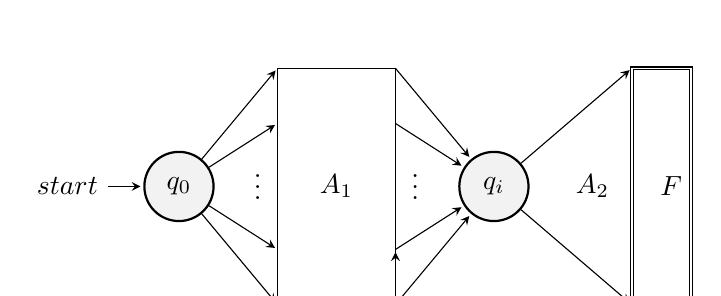
\begin{tikzpicture}[shorten >=1pt,node distance=2cm,on grid,auto]
            \node[state,initial]           (q0) {$q_0$};
            \node[right=2cm of q0]       (a1) {$A_1$};
            \node[state,right=2cm of a1] (q)  {$q_i$};
            \node[right=1.25cm of q]          (a2) {$A_2$};
            \node[right=1cm of a2]         (f)  {$F$};
          
            \coordinate[above right=1.5cm and 1.25cm of q0] (a1ul);
            \coordinate[below right=1.5cm and 1.25cm of q0] (a1bl);
            \coordinate[above right=0.8cm and 1.25cm of q0] (a1ul2);
            \coordinate[below right=0.8cm and 1.25cm of q0] (a1bl2);
            \coordinate[above right=1.5cm and 2.75cm of q0]  (a1ur);
            \coordinate[below right=1.5cm and 2.75cm of q0]  (a1br);
            \coordinate[above right=0.8cm and 2.75cm of q0]  (a1ur2);
            \coordinate[below right=0.8cm and 2.75cm of q0]  (a1br2);
            \draw (q0) edge[above] node{} (a1ul)
                  (q0) edge[below] node{} (a1bl)
                  (q0) edge[above] node{} (a1ul2)
                  (q0) edge[below] node{} (a1bl2)
                  (a1ur) edge[above] node{} (q)
                  (a1ur2) edge[above] node{} (q)
                  (a1br) edge[above] node{} (q)
                  (a1br2) edge[above] node{} (q);
            \node[above right=0.1cm and 1cm of q0] {$\vdots$};
            \node[above right=0.1cm and -1cm of q] {$\vdots$};

            \coordinate[above right=1.5cm and 1.75cm of q]  (a2o);
            \coordinate[below right=1.5cm and 1.75cm of q]  (a2u);
            \coordinate[right=0.75cm of a2o] (a2oo);
            \coordinate[right=0.75cm of a2u] (a2uu);
          
            \draw (a1ul)  -- (a1bl) -- (a1br) -- (a1ur) -- cycle;
            \draw (q) edge[above] node{} (a2o)
                  (q) edge[below] node{} (a2u);
          
            \draw[double] (a2o) -- (a2oo) -- (a2uu) -- (a2u) -- cycle;
          \end{tikzpicture}
        \end{figure}
        \\而后我们将$q_i$复制两份(记为$q_i^s, q_i^e$), 将$q_0 A_1  q_i^e$ 与 $q_i^s  A_2$位置对换,再在$F$中的状态与$q_0$之间各增加一个$\varepsilon$转移. 对每个$q_i \in Q$, 我们都可以进行这样的变换(共有$|Q|$个),  令$F' = \{q_i^e \mid \forall q_i \in Q\}$, 最后再增加一个新的起始状态$q_0^*$, 使得$q_0^*$通过$\varepsilon$转移指向每个起始$q_i^s$.图示如下:\\
        \begin{figure}[h]
        \centering 
        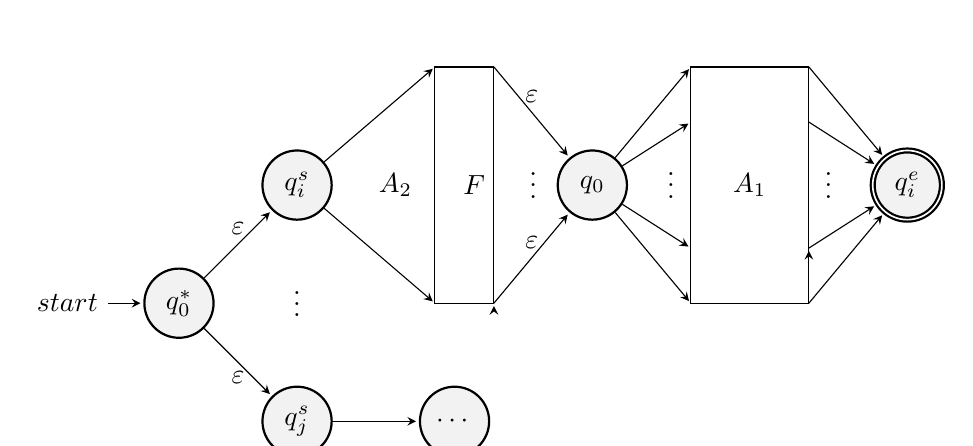
\begin{tikzpicture}[shorten >=1pt,node distance=2cm,on grid,auto]
            \node[state, initial]  (q0s) {$q_0^*$};
            \node[state, above right = 1.5cm and 1.5cm  of q0s]  (qis) {$q_i^s$};
            \node[state, above right = -1.5cm and 1.5cm  of q0s] (qjs) {$q_j^s$};
            \node[state, right = 2cm of qjs] (other) {$\cdots$};
            \node[right=1.25cm of qis]          (a2) {$A_2$};
            \node[right=1cm of a2]         (f)  {$F$};
            \node[state, right=1.5cm of f] (q0) {$q_0$};
            \node[right=2cm of q0]       (a1) {$A_1$};
            \node[state,accepting,right=2cm of a1] (qie)  {$q_i^e$};
            
            \coordinate[above right=1.5cm and 1.25cm of q0] (a1ul);
            \coordinate[below right=1.5cm and 1.25cm of q0] (a1bl);
            \coordinate[above right=0.8cm and 1.25cm of q0] (a1ul2);
            \coordinate[below right=0.8cm and 1.25cm of q0] (a1bl2);
            \coordinate[above right=1.5cm and 2.75cm of q0]  (a1ur);
            \coordinate[below right=1.5cm and 2.75cm of q0]  (a1br);
            \coordinate[above right=0.8cm and 2.75cm of q0]  (a1ur2);
            \coordinate[below right=0.8cm and 2.75cm of q0]  (a1br2);
            \draw (q0) edge[above] node{} (a1ul)
                  (q0) edge[below] node{} (a1bl)
                  (q0) edge[above] node{} (a1ul2)
                  (q0) edge[below] node{} (a1bl2)
                  (a1ur) edge[above] node{} (qie)
                  (a1ur2) edge[above] node{} (qie)
                  (a1br) edge[above] node{} (qie)
                  (a1br2) edge[above] node{} (qie)
                  (q0s) edge[above] node{$\varepsilon$} (qis)
                  (q0s) edge[below] node{$\varepsilon$} (qjs)
                  (qjs) edge[above] node{} (other);
            \node[above right=0.1cm and 1cm of q0] {$\vdots$};
            \node[above right=0.1cm and -1cm of qie] {$\vdots$};
            \node[above right=0.1cm and 0.75cm of f] {$\vdots$};
            \node[above right=0.1cm and 1.5cm of q0s] {$\vdots$};

            \coordinate[above right=1.5cm and 1.75cm of qis]  (a2o);
            \coordinate[below right=1.5cm and 1.75cm of qis]  (a2u);
            \coordinate[right=0.75cm of a2o] (a2oo);
            \coordinate[right=0.75cm of a2u] (a2uu);
            \draw (a2oo) edge[above] node{$\varepsilon$} (q0)
                  (a2uu) edge[above] node{$\varepsilon$} (q0);
          
            \draw (a1ul)  -- (a1bl) -- (a1br) -- (a1ur) -- cycle;
            \draw (qis) edge[above] node{} (a2o)
                  (qis) edge[below] node{} (a2u);
          
            \draw (a2o) -- (a2oo) -- (a2uu) -- (a2u) -- cycle;
          \end{tikzpicture}
        \end{figure} 
        \\下面我们简单证明一下$L(N) = RC(A)$.
        
        1. $\forall z \in RC(A), \exists xy \in A, ~s.t.~ z = yx$. 设$x = w_1 w_2 \cdots w_i, y = w_{i+1} w_{i+2} \cdots w_k, \delta(q_{i-1}, w_i) = q_i$.即$q_0 \overset{x}{\longrightarrow} q_i \overset{y}{\longrightarrow} q_{a} \in F$.那么对$N$, 由定义有如下的状态转移序列使得$z \in L(N)$:
        \[
          q_0^* \overset{\varepsilon}{\longrightarrow} q_i^s \overset{y}{\longrightarrow} q_a \overset{\varepsilon}{\longrightarrow} q_0 \overset{x}{\longrightarrow} q_i^e \in F'
        \]
        2. $\forall z \in L(N)$,存在一个状态序列$q_0^* \overset{\varepsilon}{\longrightarrow} q_i^s \overset{y'}{\longrightarrow} q_a \overset{\varepsilon}{\longrightarrow} q_0 \overset{x'}{\longrightarrow} q_i^e \in F' ~s.t.~ z = y'x'$. 那么对$M$, 考虑对应的状态转移序列$q_0 \overset{x'}{\longrightarrow} q_i \overset{y'}{\longrightarrow} q_{a} \in F \implies x'y' \in A \implies y'x' \in RC(A)$.
        
        因此, $L(N) = RC(A)$. 由于$N$是一个NFA, 因此$RC(A)$是一个正则语言.
    \end{enumerate}
\end{answer}
\end{document}